\section{Preliminaries}
\label{sec:prelim}

\noindent\textbf{Problem formulation.}
Our goal is to train policies $\pi(a_{1:H} \vert o)$ that map an observation $o$ to a sequence of future robot actions $a_{1:H}$. We assume that policies output an ``action chunk''~\cite{zhao2023learning,laiaction}, a \emph{sequence} of $H$ actions~\citep{chi2023diffusionpolicy,black2024pi_0,zhao2023learning}, which makes it easier to produce temporally-consistent actions and reduces compounding error. The goal of \textit{action tokenization} is to define a mapping $\mathcal{T}_a: a_{1:H} \rightarrow [T_1, \dots, T_n]$
from a sequence of continuous actions $a_{1:H}$, with dimensionality $\vert \mathcal{A}\vert$, to a sequence of $n$ discrete tokens $T \in \vert \mathcal{V}\vert$ from a vocabulary of size $\vert \mathcal{V}\vert$. Note that the number of tokens $n$ may differ between action sequences, just like sentences of the same length may be tokenized into a variable number of text tokens. 

\noindent\textbf{Binning-based action tokenization.}
The most commonly used approach for action tokenization is a simple binning discretization scheme~\citep{rt12022arxiv,rt22023arxiv,kim2024openvla,zhen20243dvla,reed2022generalist}. For a given action $a$, this approach discretizes each dimension independently, dividing the range of values in the training dataset into $N$ uniform bins, most commonly using $N=256$. For a \emph{sequence} of $D$-dimensional actions $a_{1:H}$, this tokenization scheme would be applied to each time step, resulting in a final token sequence $\mathcal{T}_a\big(a_{1:H}\big) = [T_{1, 1}, \dots, T_{1, D}, \dots, T_{H, 1}, \dots, T_{H, D}]$. For high-frequency robot data, this tokenization scheme is sub-optimal: it can easily produce hundreds of tokens per action chunk, which make training challenging and lead to slow inference.

\section{Case Study: How Does Tokenization Affect VLA Training?}
\label{sec:educational_example}

\begin{figure}
    \centering
    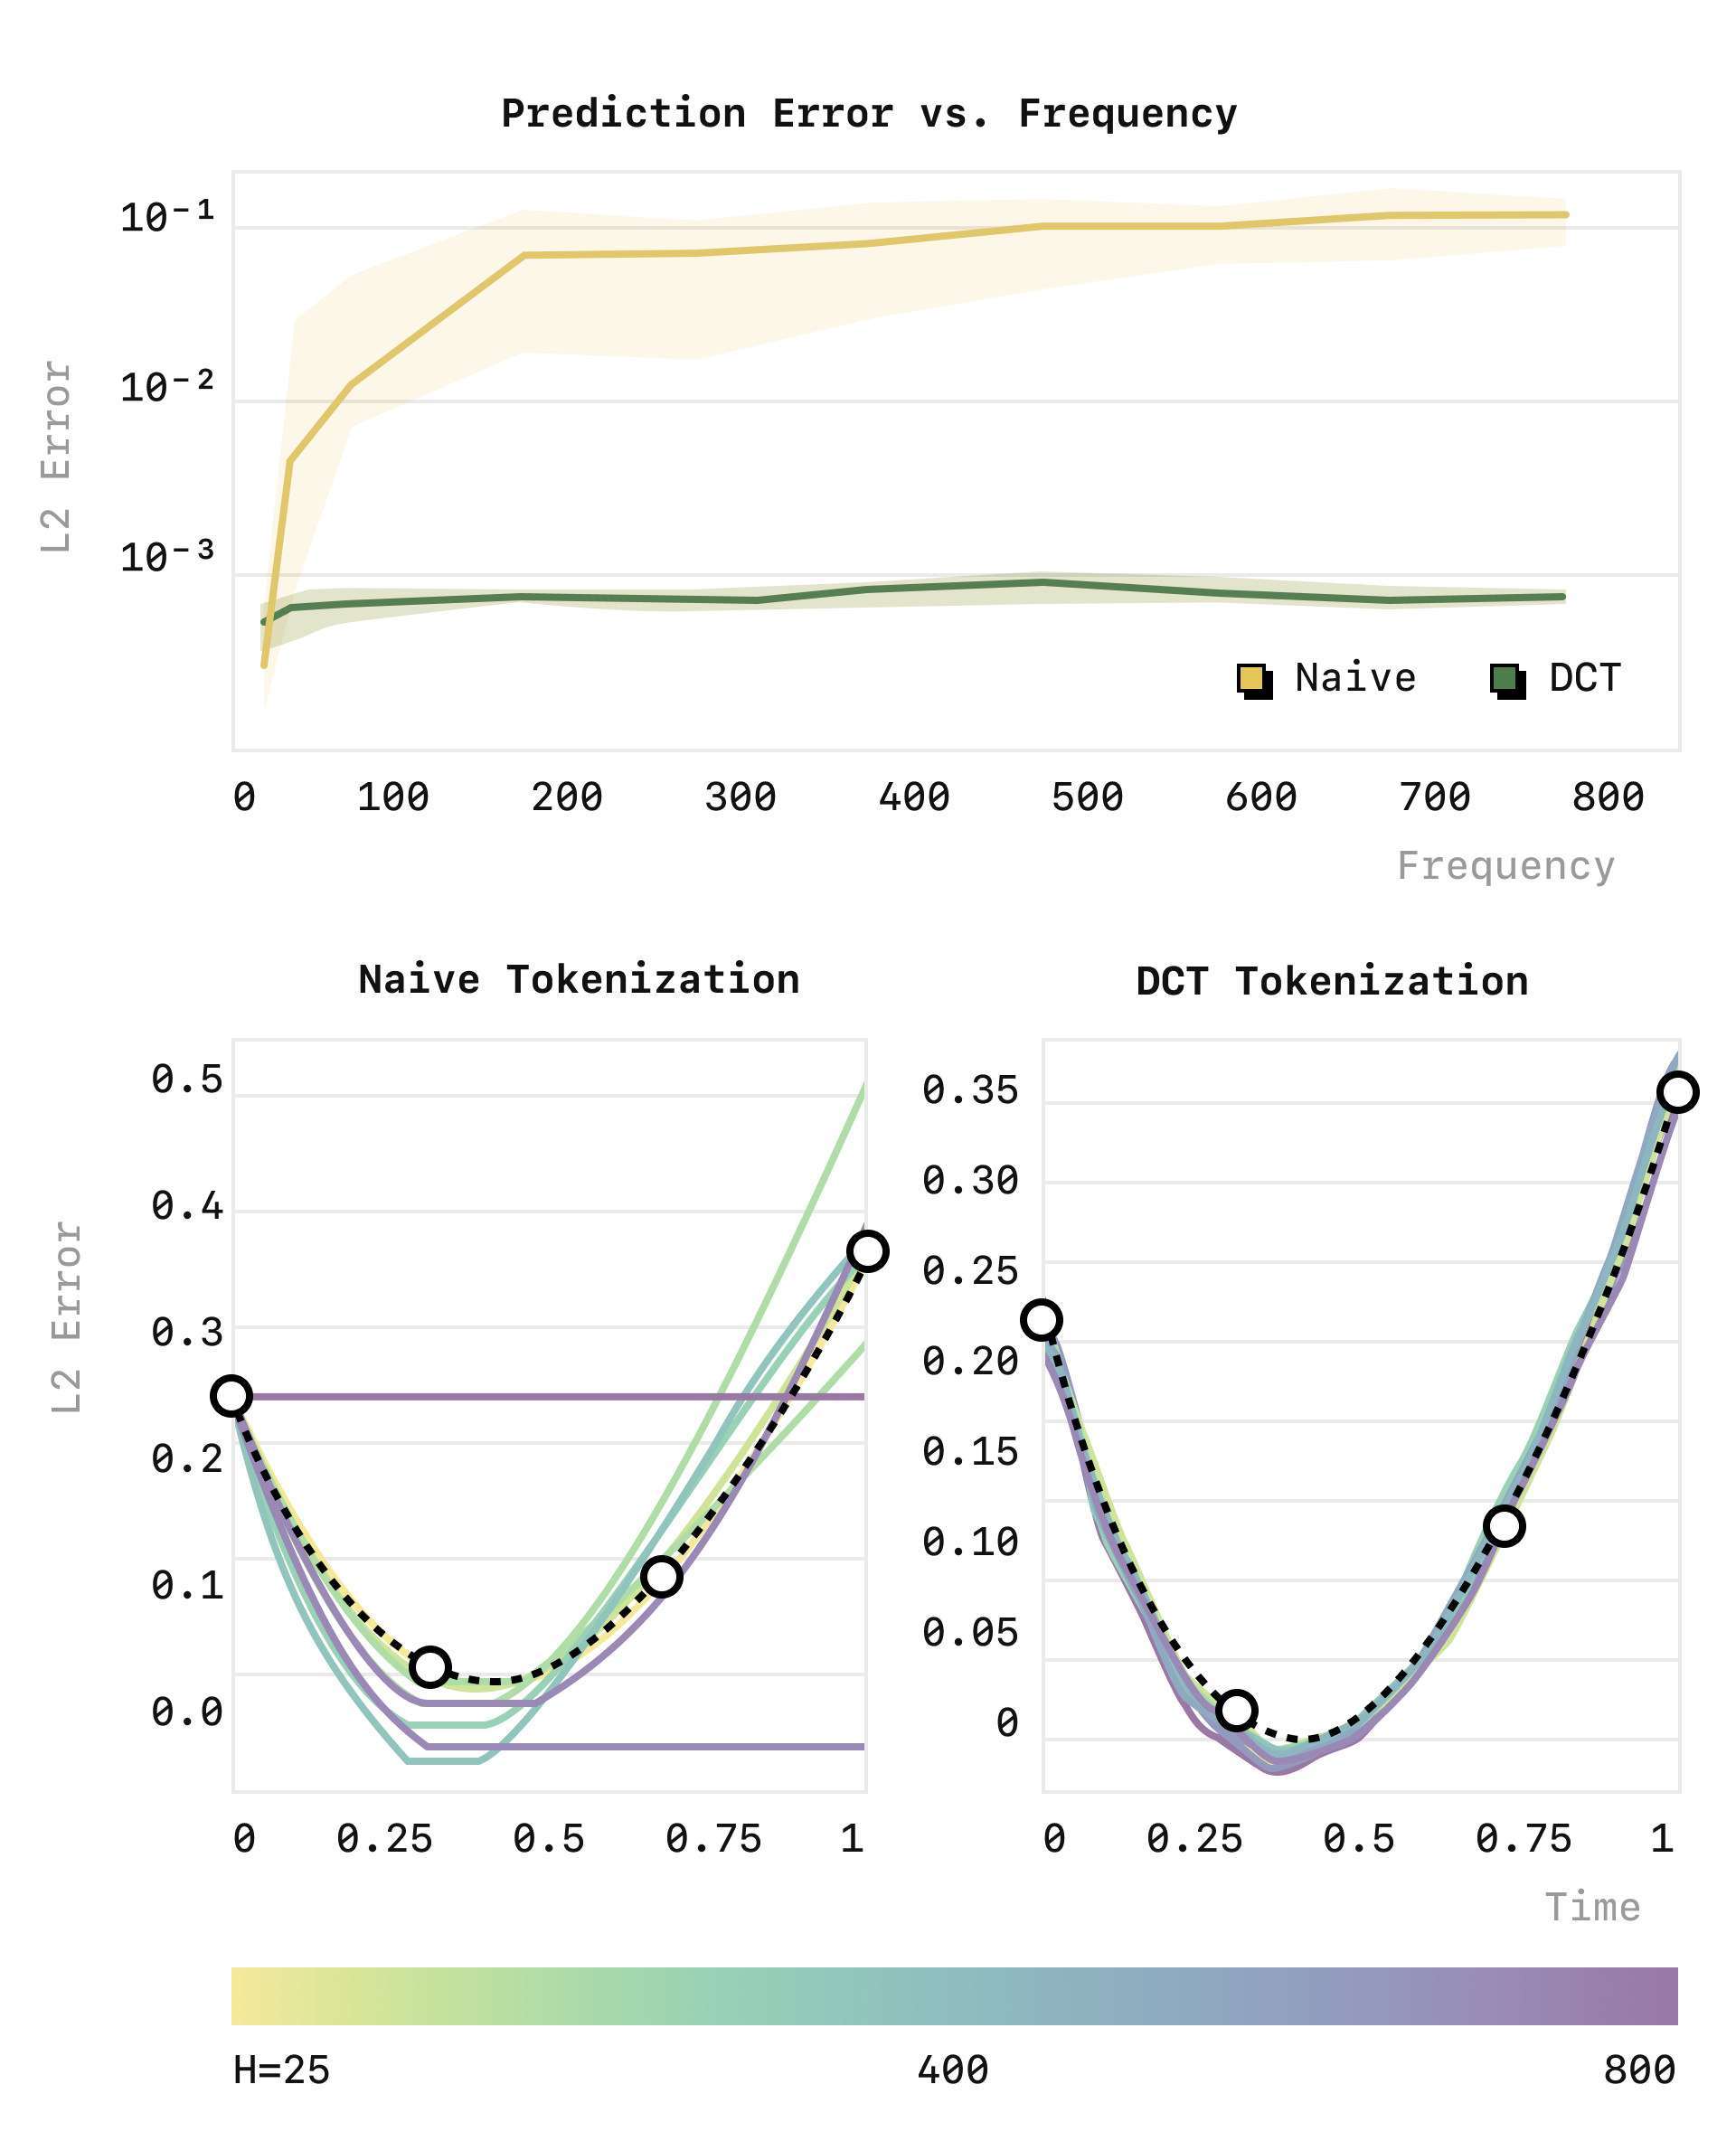
\includegraphics[width=\linewidth]{figures/case_study.png}
    \caption{\textbf{Effect of sampling rate on prediction performance.} We train a small autoregressive transformer model on a didactic interpolation task, in which the network must predict the black dashed curve given the four circles. 
    We find that models trained with the binning tokenization approach used in prior VLAs~\cite{rt22023arxiv, kim2024openvla} produce increasingly poor predictions as we increase the sampling frequency of the underlying signal, due to strong correlation between consecutive tokens at high frequencies. Our \ModelAcronym{} tokenization approach, based on the discrete cosine transform (DCT), addresses the problem and leads to high-quality predictions across all sampling rates.
    }
    \label{fig:toy_example}
\end{figure}

To illustrate the challenge of training autoregressive policies with current action tokenization approaches, we start with a simple didactic example. We create a synthetic time-series dataset where the goal is to predict a cubic spline that interpolates four randomly-generated points (see \cref{fig:toy_example}, bottom). This toy problem reflects the challenge faced by policies trained on high-frequency action chunks, which must predict a sequence of continuous actions given some conditioning information. We tokenize the target sequences using the na\"{i}ve tokenization scheme employed in previous VLA policies, which discretizes each element in the sequence separately into one of 256 bins (see \cref{sec:prelim}). We then train a small, autoregressive transformer policy to predict the tokenized signal given the conditioning points. We repeat this experiment for different \emph{sampling rates} of the target signal, from 25 to 800 timesteps per sequence, without changing the underlying dataset. This emulates training autoregressive policies on action data collected at different frequencies.

The average prediction MSE of autoregressive models trained at different frequencies is shown in \cref{fig:toy_example}, top (``naive'').
We observe that the model with binning tokenization achieves good prediction performance (i.e., low MSE) for low sampling rates. But as the sampling rate increases, the prediction error steeply increases, until eventually the model simply copies the first action, as seen in the qualitative visualization in \cref{fig:toy_example}, bottom left. Note that this issue \emph{cannot} be attributed to the data itself: the complexity of the underlying data distribution does not change, and we would expect a model with the same capacity trained for the same number of steps to achieve comparable performance across all sampling rates. %
So what happened?

To understand how the tokenization scheme impacts learning performance, we need to look at the learning objective itself. Fundamentally, autoregressive models are trained to predict the next token, given all previous tokens. As such, their learning signal is proportional to the marginal information content of $T_i$ given $T_{1:i-1}$. Crucially, when using the na\"{i}ve per-timestep tokenization scheme, this marginal information \emph{approaches zero} as the control frequency of the training signal increases: for smooth signals, as timesteps get shorter the change per timestep decreases proportionally.
This greatly \emph{slows down} the rate of convergence during training and can make it challenging to fit complex, high-frequency datasets. Indeed, such challenges have been observed in prior work. For instance, OpenVLA worked well on the low-frequency BridgeV2 and RT-1 datasets, but has struggled to fit the higher-frequency DROID dataset~\citep{kim2024openvla}. The result of our case study underlines the importance of designing better tokenization schemes for robot actions.
